\documentclass[a4paper, 12pt]{article}

\usepackage[swedish]{babel}
\usepackage[T1]{fontenc}
\usepackage[utf8]{inputenc}
\usepackage{amsmath}
\usepackage{graphicx}
\usepackage{fancyhdr}
\usepackage{csquotes}
\usepackage{tikz}
\usepackage{pgfplots}
\usepackage{lmodern}
\usepackage{float}

\usepackage[style=authoryear-ibid,backend=biber]{biblatex}

\addbibresource{sources.bib}% Syntax for version >= 1.2

\pagestyle{fancy}

{\fontfamily{qcr}\selectfont

\lhead{Tomass Wilson}
\rhead{Grupp B:7}
\renewcommand{\headrulewidth}{0.4pt}
\renewcommand{\footrulewidth}{0.4pt}

\title{Bestämmande av optimal arkitektur för artificiella neuronnät med evolution}
\author{Tomass Wilson\\thmwi@kth.se\\Grupp B:7}

\begin{document}

  \pagenumbering{gobble}

  \maketitle

  \begin{abstract}
    Maskininlärning används mer och mer i dagens industrier och programutveckling. Utvecklingen av artificiella neuronnät bör optimeras för att underlätta applikationen av denna viktiga teknologi till allt fler och fler områden. Vid körning av Matt Harveys python program \parencite{harvey2017} syns ett tydligt sätt tiden detta tar kan förkortas. Processen kan förbättras genom användning av en evolutionär algoritm som fungerar på principerna av naturligt urval. Denna process är byggd för att bestämma det optimala neuronnätsarkitektur, då olika kombinationer av meta-variabler såsom antal neuroner och optimeringsfunktion kan starkt påverka nätverkets träffsäkerhet och inlärningstid. Algoritmen testar flera kombinationer, men undviker onödiga tester genom att simulera 20 neuronnät i en population genom flera generationer. Undersökningen visar på förbättringar på gentemot iterativ sökning, då processtiden vid denna studie gick från 18 till 3 timmar, en förbättring av 80 \%. Detta kan appliceras på flera olika implementeringar av artificiella neuronnät för att förenkla och effektivisera deras utveckling.
  \end{abstract}

  \newpage

  \pagenumbering{roman}

  \tableofcontents

  \newpage

  \pagenumbering{arabic}

  \section{Inledning}
    Genom tiden har programmerare alltid försökt lösa svårare problem. När Artificiella Neuronnät (ANN) började utvecklas kunde man applicera dem på problem som fördetta verkade omöjliga, såsom att urskilja ansikten eller kategorisera bilder \parencite{hopfield1988artificial}. Inlärningsprocessen tar ofta flera timmar och bygger på att slumpa fram de kopplingarna mellan neuroner sådan att en viss träffsäkerhet på resultatet nås för det specificerade problemet. En viktig faktor som påverkar inlärningen av ett ANN är meta-variabler, såsom antal neuroner per lager, antal lager, aktiveringsfunktionen, etcetera. Dessa meta-variabler kan ställas in manuellt av användaren, men detta brukar leda till att neuronnätet inte når sin maximala träffsäkerhet, eller förlänger inlärningstiden märkbart. Lösningen till detta har tidigare varit att iterera genom alla möjliga kombinationer meta-variabler och testa dem var för sig. En föreslagen lösning till detta är att istället evolutionärt optimera slumpmässigt valda meta-variabler för att undvika onödiga tester av ineffektiva kombinationer av dessa.

    \subsection{Syfte}
    Syftet med denna studie är att undersöka om tiden för inlärandeprocessen för ett neuralt nätverk kan förkortas med hjälp av en evolutionär process. Precisionen för nätverket ska vara helst den samma som vid en iterativ inlärningsprocess, för att kunna ge en komparabel alternativ.
    \subsection{Frågeställning}
    Kan den evolutionära metoden av Matt Harveys pythonprogram uppskatta de optimala meta-variablerna på kortare tid än en iterativ sökning?

  \section{Bakgrund \& Teori}
    \subsection{CIFAR-10}
    Industri-standarden för att testa ANN är CIFAR-10, en databas av 60 000 bilder, som kategoriseras in i 10 grupper \cite{krizhevsky2014cifar}. Med detta kan man okomplicerat jämföra olika ANN, genom att mäta hur snabbt och väl de kan identifiera vilken kategori en bild tillhör. Som input får nätverket en bild med 32 x 32 pixlar, som mäts in ett input lager som en matris. Outputlagern har 10 neuroner, med ett värde mellan 0 och 1 för att visa hur mycket bilden ”passar” in i en viss kategori. Träffsäkerheten mäts som andel gånger neuronnätet har placerat bilden i korrekt kategori.

    \subsection{Artificiella Neurala Nätverk}
    Ett Artificiell Neural Nätverk (ANN) \parencite{hopfield1988artificial} är en samling sammankopplade neuroner sammanställda i flera \textit{lager}. Varje nod har ett värde och en aktiveringsfunktion, och befinner sig i ett lager. En nod har flera inkommande länkar och utgående länkar till andra neuroner i lager under och över den respektive. Inkommande värden multipliceras med en slumpmässig vikt och sedan multipliceras alla inkommande värden tillsammans. Detta nya värde normaliseras sedan ner till ett värde mellan 0 och 1. Denna process kallas \textit{aktiveringsfunktionen} och slutgiltiga resultatet är nodens \textit{värde}. Antal neuroner i input- och outputlagern bestäms i förhand beroende på hur nätverket ska användas. I denna studie är inputlagern en matris med 32x32 neuroner som representerar en svartvit bild, där ett högre värde (1) representerar vit och ett lägre (0) svart. Outputlagern uppbyggs av 10 neuroner, där neuronen med högsta värde representerar nätverkets \textit{gissning} för vilket kategori bilden passar in i. Till en början är alla neuronkopplingar och deras vikter slumpmässigt valda, vilket gör att den ger helt slumpmässiga svar. För att optimera nätverket krävs en \textit{optimeringsfunktion}.

    \subsection{Meta-variabler}
    För att ett ANN ska kunna skapas behövs några startparametrar. Dessa \textit{meta-variabler} bestämmer övergripande hur nätverket ser ut, dess storlek och konstruktion. Undersökningen som beskrivs i denna artikel kommer att behandla dessa meta-variabler:
    \begin{enumerate}
        \item \# Neuroner
        \newline
        Detta är antal individuella neuroner i varje lager. Detta experiment kommer testa värdena 64, 128, 256, 512, 768 och 1024 neuroner per lager.
        \item \# Lager
        \newline
        Detta är antal lager exklusive input- och outputlagern, dessa heter \textit{gömda lager} och antalet som testats i denna studie är 1, 2, 3 eller 4.
        \item Aktiveringsfunktion
        \newline
        Det existerar flera olika sorters aktiveringsfunktioner som används inom ANN i dagsläget. De har olika appliceringsområden men alla fungerar på principen att normalisera summan av alla inkommande värden till ett värde mellan 1 och 0. Vilken aktiveringsfunktion man använder påverkar hur komplex ett nätverk kan bli och dess maximala träffsäkerhet \parencite{jain1996artificial}. Detta experiment använder sig av aktiveringsfunktionerna: \textit{sigmoid, tanh} \parencite{karlik2011performance}, \textit{Exponential Linear Unit} (ELU) \parencite{clevert2015fast} och \textit{Rectified Linear Unit} (ReLU) \parencite{xu2015empirical}
        \item Optimeringsfunktion
        \newline
        Optimeringsfunktionen är den process som nätverket använder för att optimeras. Optimeringsfunktioner förbättrar nätverket genom att ändra på kopplingar och dess vikter mellan neuroner och mäta förändringen i träffsäkerhet, och behåller bara de ändringar som är gynnsamma \parencite{TypesofO34:online}. Funktionerna som ska testas är: \textit{rmsprop, sgd, adam, adagrad, adadelta, adamax } och \textit{nadam} \parencite{kingma2014adam}
    \end{enumerate}


    \subsection{Evolutionär Inlärningsprocess}
    Som i naturen fungerar den evolutionära algoritmen som ett slags naturligt urval. Vid första början skapas en population med ett visst antal neurala nätverk med slumpmässigt valda meta-variabler. Varje nätverk får sedan påbörja inlärningsprocessen, tills inlärningen når ett lokalt maximum och kan inte lära sig något mer. Tiden inlärningen tar och nätverkets träffsäkerhet mäts och kombineras, vilket då blir nätverkets \textit{fitness}. Nätverket i populationen som har lägst fitness, ”dödas” och ersätts av nätverk som är en kombination av 2 levande nätverk, ”föräldrarna”, och får sedan en slumpmässig mutation (detta för att populationen inte ska bli för homogen). Efter flera \textit{generationer} har förmodligen det bästa nätverket en sammanställning meta-variabler som är optimerade för användningsområdet. \parencite{yao1997new}

    I denna undersökning kommer systemet utföra 10 generationer, med 20 neuronnät var. Varje generation kommer undersökas och sedan kommer det 12 sämsta neuronnät (de med lång inlärningstid eller dålig träffsäkerhet) raderas (+- några, för att populationen inte ska bli homogen).  Nya nät skapas för att få populationen upp till 20 genom att slumpmässigt välja meta-variabler från två existerande nät. Sist så ändras en meta variabel helt slumpmässigt (en mutation).


\newpage

  \section{Metod}
  Tidigare studier har undersökt möjligheten av att använda evolutionära algoritmer för val av meta-variabler, såsom \textcite{yao1997new}, men det krävs fler jämförelser med existerande metoder. Detta på grund av hur ung forskningsområdet är och den höga hastigheten nya algoritmer utvecklas. Därför används denna experimentella metoden för undersökningen. För att jämföra de två olika metoder för att bestämma bästa meta-variabler användes CIFAR-10 databasen för inputmaterial. Själva processen av populationskapande, fitness evaluering och evolution är skriven av Matt Harvey \parencite{harvey2017} med några modifieringar för att spara minne gjord av Tomass Wilson. All kod skrevs i python 3.6 och kördes på Windows 10, och använder sig till huvuddel av keras och tensorflow paketen för att optimera och skapa neuronnäten. Versionerna av samtliga paket ses i tabell \ref{paketversioner}. Hårdvaran som användes i denna undersökning ses i tabell \ref{hårdvara}.

    Först testades den iterativa processen genom att köra brute.py filen. Alla 672 möjliga kombinationer meta-variabler testades och en slutsiffra på tiden hela processen tog antecknades. Detta ger en basnivå som kan jämföras med den evolutionära processen. Sedan kördes den evolutionära processen med 10 generationer av 20 neuronnät var genom att köra main.py filen, och tiden skrevs ned.


\begin{table}[H]
    \centering
    \begin{tabular}{c|c}
      Paket & Version \\
      \hline
      keras & 2.2.2 \\
      keras-applications & 1.0.4 \\
      keras-preprocessing & 1.0.2 \\
      numpy & 1.15.1 \\
      scipy & 1.1.0 \\
      six & 1.11.0 \\
      tensorflow & 1.10.1 \\
      tqdm & 4.25.0 \\
      werkzeug & 0.14.1 \\
      wheel & 0.31.1
    \end{tabular}
    \caption{Paketversioner}
    \label{paketversioner}
\end{table}

\begin{table}[H]
    \centering
    \begin{tabular}{c|c}
      Komponent & Specifikation \\
      \hline
      GPU: & RTX 2080 @ 1950 MHz core, 7263 MHz mem \\
      CPU: & Intel i7 8700 @ 4.28 GHz \\
      Minne: & 32 GB @ 2666 MHz \\
    \end{tabular}
    \caption{Hårdvara}
    \label{hårdvara}
\end{table}

  \section{Resultat}

  Dessa resultat insamlades över flera dagar, och datorn programmet kördes på användes lätt under den tiden. Detta innebär att vid vissa tillfällen kan grafikminne och grafikprocessorkraft vara erlagd på andra datorprogram under undersökningens gång. Dock så sker det mesta av denna programs uträkningar på RTX tensorkärnor vilka används inte av andra program.

  Programmet slutar med att presentera de fem bästa neuronnät som den kunde hitta. Resultatet från den evolutionära processen visas i tabell \ref{evo}, och för den iterativa i tabell \ref{iterativ}. Totala tiden för den evolutionära algoritmen samt iterativa ses i tabell \ref{total}.

\begin{table}[H]
    \centering
    \begin{tabular}{c|c|c|c|c}
      Träffsäkerhet & \#Neuroner & \#Lager & Akt-funk. & Opt-funk. \\
      \hline
      56,12 \% & 256 & 4 & ELU & adamax \\
      55,75 \% & 256 & 4 & ELU & adamax \\
      55,65 \% & 512 & 4 & ELU & adamax \\
      55,64 \% & 256 & 4 & ELU & adamax \\
      55,57 \% & 256 & 4 & ELU & adamax \\
    \end{tabular}
    \caption{5 bästa neuronnät efter evolutionär sökning.}
    \label{evo}
\end{table}

\begin{table}[H]
    \centering
    \begin{tabular}{c|c|c|c|c}
        Träffsäkerhet & \#Neuroner & \#Lager & Akt-funk. & Opt-funk. \\
        \hline
        55,52 \% & 768 & 2 & ELU & adamax \\
        55,47 \% & 1024 & 2 & ELU & adamax \\
        55,33 \% & 512 & 3 & ELU & adamax \\
        55,30 \% & 768 & 2 & sigmoid & adamax \\
        55,21 \% & 768 & 4 & sigmoid & adamax \\
    \end{tabular}
    \caption{5 bästa neuronnät efter iterativ sökning.}
    \label{iterativ}
\end{table}

\begin{table}[H]
    \centering
    \begin{tabular}{c|c|c}
      Inställning & Tid & Maximal Träffsäkerhet\\
      \hline
      Evolutionär: & 3 h 43 m 14 s & 56,12 \% \\
      Iterativ: & 18 h 53 m 40 s & 55,52 \% \\
    \end{tabular}
    \caption{Total tid för hela processen}
    \label{total}
\end{table}

\newpage

För att få ett närmare inblick i den evolutionära processen så kördes den i flera omgångar och träffsäkerhet för varje omgång/generation presenteras i figur \ref{generation}.

\begin{figure}[H]
\centering
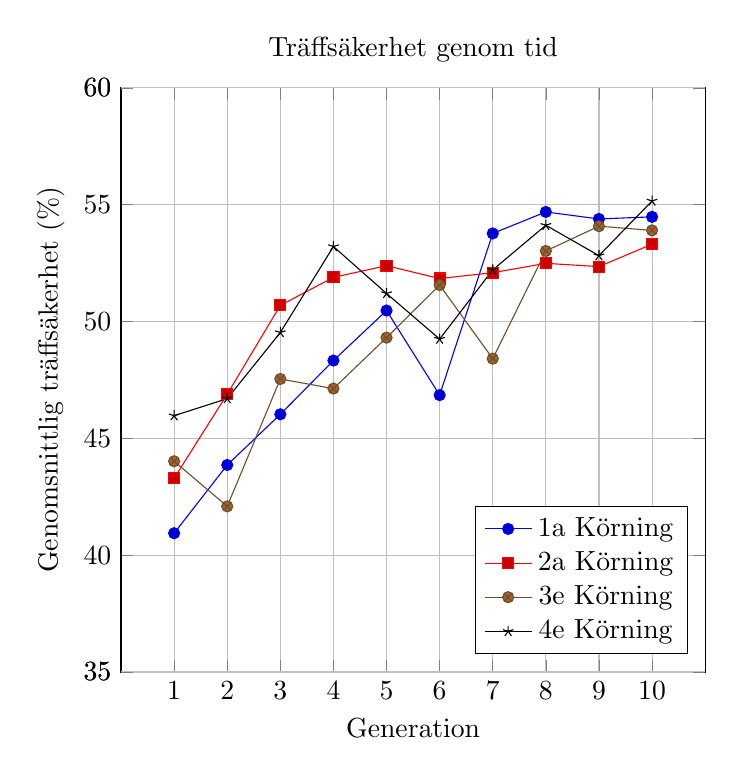
\begin{tikzpicture}
	\begin{axis}[
		height=9cm,
		width=9cm,
		grid=major,
        legend pos=south east,
        title=Träffsäkerhet genom tid,
        xlabel=Generation,
		ylabel=Genomsnittlig träffsäkerhet (\%),
        xmin=0,   xmax=11,
    	ymin=35,   ymax=60,
    	xtick={1,2,...,10},
    	extra y ticks={35,60},
	]

	\addplot coordinates {
        (1, 40.94)
        (2, 43.86)
        (3, 46.03)
        (4, 48.33)
        (5, 50.47)
        (6, 46.85)
        (7, 53.77)
        (8, 54.69)
        (9, 54.39)
        (10, 54.48)
	};
	\addlegendentry{1a Körning}

    \addplot coordinates {
        (1, 43.29)
        (2, 46.89)
        (3, 50.69)
        (4, 51.89)
        (5, 52.39)
        (6, 51.84)
        (7, 52.09)
        (8, 52.49)
        (9, 52.35)
        (10, 53.31)
	};
	\addlegendentry{2a Körning}

    \addplot coordinates {
        (1, 44.02)
        (2, 42.09)
        (3, 47.54)
        (4, 47.13)
        (5, 49.31)
        (6, 51.56)
        (7, 48.41)
        (8, 53.02)
        (9, 54.08)
        (10, 53.90)
	};
	\addlegendentry{3e Körning}

    \addplot coordinates {
        (1, 45.97)
        (2, 46.70)
        (3, 49.53)
        (4, 53.21)
        (5, 51.20)
        (6, 49.25)
        (7, 52.21)
        (8, 54.12)
        (9, 52.82)
        (10, 55.16)
	};
	\addlegendentry{4e Körning}

	\end{axis}
\end{tikzpicture}
\caption{Träffsäkerhet för varje generation}
\label{generation}
\end{figure}


  \section{Diskussion}
    Enligt resultatet som redovisas i tabell \ref{total} så kan frågeställningen enkelt besvaras. En skillnad på 15 timmar 10 minuter visar på den stora fördelen med att använda den evolutionära processen Samtidigt som träffsäkerheten behålls inom användbara ramer. Detta motsvara en förkortning av 80,3 \% av inlärningstiden Däremot måste implementationen av systemet diskuteras samt hur applicerbart detta är på andra datamängder/maskininlärningsproblem. Studien som genomfördes riktar sig in på bara ett av flera andra problem som maskininlärning appliceras på. Vissa användningar, där neuronnätets arkitektur är given eller inlärningstiden är väldigt kort behövs inte sådana metoder, då den bara försvårarar för användaren. Åt andra sidan så kan detta system underlätta för sökandet av meta-variabler då dessa är okända, och kommer troligen ge nästan lika bra output som en iterativ process.

    Bästa nätverket som hittades i första evolutionära körning (tabell \ref{evo}) är inte den samma som den som hittades av den iterativa processen (tabell \ref{iterativ}). Detta är inte ett stort problem, då de fick nästan samma maximala träffsäkerhet, men de kan ha olika inlärningstid. Totala antalet neuroner är väldigt lika, $256 * 4 = 1024$ medans $768 * 2 = 1536$, vilket tyder på olika lösningar till lika problem. Dessutom, eftersom optimeringsprocessen utgår ifrån att slumpmässigt försöka förbättra varje neuronnät, så kan man få olika träffsäkerhet vid varje optimeringsomgång för \textit{samma} sammanställning meta-variabler. Däremot kommer någon avvikning vara liten och inte spela mycket roll även om det leder till att man väljer än eller annan arkitektur för neuronnätet, då träffsäkerheten är viktigast. Om det absolut bästa sammanställning meta variabler är nödvändigt, kan processen köras flera gånger och det neuronnät som har konsekvent bäst träffsäkerhet kan användas.

    Genom att granska resultatet i figur \ref{generation} kan det synas hur vid varje omgång så förbättras populationen från en slumpmässig sammanställning neuronnät vid första generation till en population där nästa alla individer är av samma, effektiva design (från ~45 \% till ~55 \%). Även om vid tillfällen med fler/olika meta-variabler så kräver den evolutionära processen fler generationer och större populationer för att klara av samma förbättring, så kommer den iterativa processen alltid att behöva gå igenom alla kombinationer vilket då leder till att den evolutionära processen ger stora tidsfördelar med nästan samma resultat i det flesta fall.


  \subsection{Felkällor}

  En fällkälla som uppstår vid denna undersökning är att datorn kan inte alltid leverera samma prestanda vid alla tillfällen, särskilt om den används under samma tid. Dock är detta systematiskt för båda processen, och skillnaden är troligen så liten att den inte kunde påverka resultaten.

  \subsection{Fortsatta studier}

  Fler studier bör göras med andra sammanställningar meta-variabler och fler omgångar, för att testa den evolutionära processen med svårare starttillstånd. Det är troligt att vid denna studie fanns ett få antal optimala neuronnät (träffsäkerhet på 54–55 \%) existerande redan i populationen för första generationen. En intressant framtida undersökning skulle kunna testa om det evolutionära systemet kan utveckla det optimala kombination bara med hjälp av naturligt urval, istället för att bara ”sprida” det effektivast neuronnät genom populationen.

  \subsection{Slutsats}

  Slutsatsen för denna studie är att en evolutionär process för urval av meta-variabler kan kraftigt förkorta tiden det krävs för en sådan sökning. Vid tillfällen med långa inlärningstider/stort antal meta-variabler lönar sig metoden mest, och den kan öppna dörrar för nya appliceringar av maskininlärning där förut utvecklingstiden har varit ett hinder för programmerare.

\addcontentsline{toc}{section}{Referenser}

\printbibliography

\end{document}
